% SPDX-License-Identifier: CC-BY-SA-4.0
% SPDX-FileCopyrightText: Louis Royer <infos.louis.royer@gmail.com>
\documentclass[../main.tex]{subfiles}
\begin{document}
\initSubfile[5]
\dummylabel{sec:ULCL}{2.2.2.1}
\dummylabel{sec:SR4MEC-One-Big-Upf}{3.2.2}
\dummylabel{sec:edge-policy}{3.3}
\dummylabel{sec:edge-instance-rebinding}{3.4.2}
\dummylabel{ch:mobility}{4}
\dummylabel{sec:mobility-with-immediate-intance-update}{4.3.2}

\chapter{Plateforme d'expérimentation et évaluation}
\label{ch:testbed}

\begin{chapterHeader}
Dans ce chapitre, nous présentons notre plateforme d’expérimentation libre et open-source qui permet le déploiement d’un \gl{CN}{cœur de réseau}~5G non simulé et de \gl{RAN}{réseaux d’accès} émulés ou réels.
Nous avons implémenté notre architecture~SR4MEC au sein de cette plateforme, et y avons également intégré plusieurs implémentations d’\gl{UPF}{UPF}~5G classiques.
Nous montrons que les composants créés pour cette thèse sont interopérables avec des composants d’implémentation tierce.
Nous utilisons cette plateforme pour évaluer notre architecture~SR4MEC, la comparer à une architecture~5G classique, et la tester dans des scénarios de mobilité.
\end{chapterHeader}

\section{Plateforme d’expérimentation}
\subsection{Présentation de la plateforme}
Afin de tester et valider notre proposition d’architecture intégrant des \gl{edge}{\textit{edges}} dans les réseaux~5G, nous avons développé une plateforme d’expérimentation reposant sur une infrastructure entièrement conteneurisée.
Puisque nous souhaitons confirmer l’intégration avec des réseaux~5G existants, nous devons nous appuyer sur des systèmes~5G réels plutôt que sur des modèles de simulation.
Nous adoptons une approche modulaire fondée sur des conteneurs afin de faciliter à la fois la reproductibilité des expériences, et de permettre le déploiement de composants fonctionnels pré-existants.
Cette approche nous permet de comparer notre architecture à des solutions existantes.
De plus, la diffusion de la plateforme~\cite{NEXTMN} sous une licence libre et open-source permet au reste de la communauté scientifique d’intégrer facilement de nouveaux composants et de créer leurs propres expériences.
Comme représenté sur la figure~\ref{fig:testbed}, à partir de la description de la topologie du réseau et de la définition de la politique~\textit{edge}, notre plateforme génère une spécification logicielle~\cite{COMPOSE.SPEC}~(\texttt{compose.yml}) du réseau~5G qui permet le déploiement automatisé de l’ensemble des composants sous forme de conteneurs.

\begin{figure}[h]
    \centering
    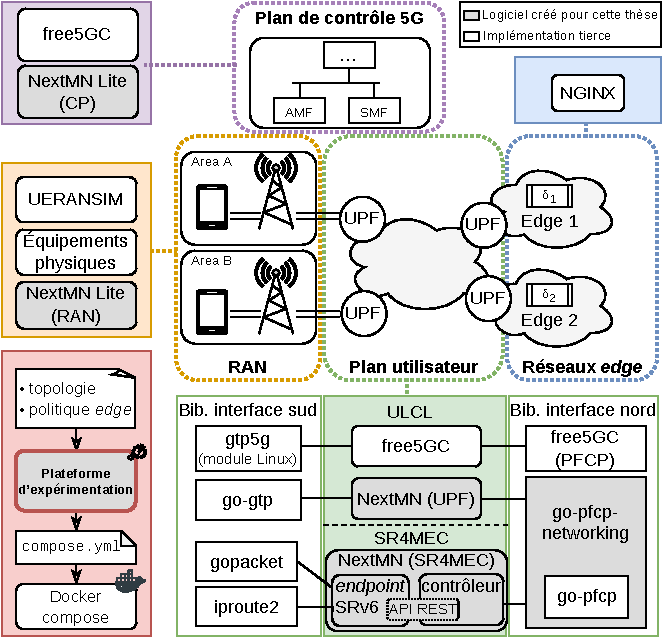
\includegraphics[width=0.75\linewidth]{figs/00_testbed.drawio.pdf}
    \caption[Vue d’ensemble de notre plateforme d’expérimentation]{Vue d’ensemble de la plateforme d’expérimentation.}
    \label{fig:testbed}
\end{figure}
\pagebreak

\subsection{Composants fonctionnels existants}
\label{sec:testbed-composants-existants}
% Intro
Nous avons intégré des composants pré-existants à notre plateforme, ce qui permet de nous rapprocher autant que possible d’un déploiement réel, et de vérifier l’interopérabilité de nos solutions.

% Cœur de réseau avec free5GC
Le projet \textbf{free5GC}~\cite{FREE5GC}, qui a rejoint la Fondation~Linux en 2024, vise à implémenter un \gl{CN}{cœur de réseau} correspondant à la \textit{release}~15 du standard.
Ce projet met à disposition sous une licence libre un ensemble de \gl{NF}{NFs}, majoritairement implémentées en Go, et utilise une \gl{SBA}{architecture basée sur des services}.
Lors de son intégration, ce projet était plus avancé dans son développement que les principales alternatives open-sources (\gl{CN}{cœurs} d’OpenAirInterface~\cite{OAI.CN} et Open5GS~\cite{OPEN5GS}), ce qui nous a conduit à l’intégrer en priorité.

Concernant le \gl{CUPS}{plan de données}, seules les \gl{PDU Session}{sessions~PDU} de type IPv4 sont implémentées: IPv6 ne figure pas encore sur la feuille de route du projet.
L’\gl{UPF}{UPF} de free5GC pilote \texttt{gtp5g}, un module du noyau Linux écrit en C, et maintenu par le projet.
Cette approche permet d’obtenir de bonnes performances pour le \gl{CUPS}{plan de données}, cependant elle rend complexe à la fois les modifications et l’installation, la compatibilité ne pouvant être assurée qu’avec un nombre restreint de versions.
Pour permettre de simplifier l’installation de la plateforme, nous avons également écrit un \gl{UPF}{UPF} en Go qui utilise les bibliothèques logicielles \texttt{go-gtp}~\cite{GO-GTP} et \texttt{go-pfcp}~\cite{GO-PFCP}, et ne fait donc pas appel à un module du noyau supplémentaire pour le traitement des \gl{PDU}{PDUs}.
Cette approche est moins performante, puisque les données sont traitées dans l’espace utilisateur et non dans l’espace noyau, mais elle facilite l’installation de la plateforme et la reproductibilité des expériences.
Lors de ce développement, nous avons mené des tests d’interopérabilité et identifié des erreurs d’implémentation dans l’\gl{UPF}{UPF} et dans le \gl{SMF}{SMF} de free5GC; nous avons envoyé des correctifs qui ont été intégrés.

% RAN
%% Compatibilité avec RAN physique
Notre plateforme est compatible avec des équipements physiques pour le \gl{RAN}{réseau d’accès}, tels qu’un \gl{RAN}{RAN} OpenAirInterface~\cite{OAI.RAN} déployé sur des \acrfrpl{USRP}, ou que d’autres équipements comme la \gl{gNB}{gNB} Amarisoft~\cite{AMARISOFT.CALLBOX}.
Cependant, la configuration de ces équipements ainsi que le routage entre les \gl{gNB}{gNBs} physiques et la plateforme reste en dehors du périmètre de la plateforme.

%% RAN émulé avec UERANSIM
Pour permettre de configurer automatiquement les \gl{UE}{équipements utilisateur} et \gl{gNB}{stations de base}, nous intégrons également des \gl{gNB}{gNB} et \gl{UE}{UEs} virtuels du projet \textbf{UERANSIM}~\cite{UERANSIM}.
Ce projet permet d’émuler les équipements du \gl{RAN}{RAN}, et implémente les protocoles de la~5G en simulant partiellement une liaison radio.
Nous avons créé deux images de conteneurs, qui permettent le déploiement de ces \gl{gNB}{gNBs} et \gl{UE}{UEs} virtuels.
Du point de vue du cœur de réseau, la \gl{gNB}{gNB} n’est pas différenciable d’un équipement physique.
Dans les conteneurs des \gl{UE}{UEs}, lors de l’établissement des \gl{PDU Session}{sessions~PDU} les adresses~IP sont ajoutées sur des interfaces~TUN (des interfaces réseau virtuelles de niveau~3).
Pour envoyer les \gl{PDU}{PDUs} vers la \gl{gNB}{gNB}, les applications présentes sur les \gl{UE}{UEs} doivent utiliser ces interfaces et adresses.

Comme pour le \gl{CN}{cœur de réseau} de free5GC, seules les \gl{PDU Session}{sessions~PDU} de type IPv4 sont implémentées pour le moment.
Le projet UERANSIM ne permet pas d’émuler la mobilité des \gl{UE}{équipements utilisateur}, nous avons donc encadré 2~stages de master visant à implémenter la procédure de \gl{handover}{\textit{handover}}~N2.

\subsection{Implémentation de l’architecture SR4MEC}
Nous avons implémenté les composants fonctionnels de notre proposition d’architecture en Go, et créé des images~OCI (Open Container Initiative~\cite{OCI}) pour les intégrer au sein de notre plateforme.
Pour rappel, le \textit{Big UPF} que nous décrivons dans la section~\ref{sec:SR4MEC-One-Big-Upf} est constituée d’un \gl{controller}{contrôleur} et de routeurs implémentant un ensemble de comportements~\gl{SRv6}{SRv6}.

Pour son interface nord, le \gl{controller}{contrôleur} utilise \texttt{go-pfcp}, la même bibliothèque logicielle que pour notre implémentation d’\gl{UPF}{UPF} classique.
Les règles~\gl{PFCP}{PFCP} obtenues sont traduites en règles de routage~\gl{SR}{SR}, puis configurées par l’interface sud en utilisant une \gl{API}{API}~\gl{REST}{REST} minimaliste.
La politique~\textit{edge} est gérée directement dans le \gl{controller}{contrôleur}, et peut être spécifiée au moyen d’un fichier de configuration.

Les routeurs~\gl{SR}{SR} implémentent les comportements~\gl{SRv6}{SRv6}~\gl{MUP}{MUP} dans l’espace utilisateur sous forme de \gl{VNF}{fonctions réseau virtuelles} en utilisant la bibliothèque \texttt{go-packet}~\cite{GOPACKET}.
Cette approche est moins performante que l’écriture d’un module du noyau ou d’un programme~eBPF, mais elle permet d’aboutir plus facilement à un premier prototype.
Les autres comportements~\gl{SRv6}{SRv6} déjà implémentés par le noyau~Linux sont configurés en utilisant l’utilitaire~\texttt{iproute2}.
Les routeurs embarquent un serveur~HTTP léger pour exposer l’\gl{API}{API}~\gl{REST}{REST} qui permet de mettre à jour les règles de routage dynamiquement.

\subsection{Gestion de la mobilité}
Dans l’objectif de valider expérimentalement la gestion de la mobilité par l’architecture que nous proposons, nous devons d’une part utiliser des \gl{gNB}{gNBs} et \gl{UE}{UEs} qui implémentent la procédure de \gl{handover}{\textit{handover}}~N2, et d’autre part parvenir à initier le \gl{handover}{\textit{handover}}.
Même si le \gl{handover}{\textit{handover}}~N2 peut théoriquement être déclenché à l’initiative du \gl{CN}{cœur de réseau}, c’est-à-dire sans attendre un message \texttt{Handover~Required} au préalable, free5GC ne permet pas d’initier le \gl{handover}{\textit{handover}}~N2 de cette manière.
Lorsque des équipements physiques sont utilisés, il est possible d’adapter les seuils de puissance du signal puis de déplacer physiquement l’\gl{UE}{UE}.
Cette méthode rend les expériences complexes à reproduire, et limite le nombre de \gl{handover}{\textit{handovers}} réalisables lors de nos mesures.
Nous choisissons donc d’utiliser une solution d’émulation du \gl{RAN}{RAN} plutôt que des équipements physiques.

Comme indiqué dans la \hyperref[sec:testbed-composants-existants]{section précédente}, la procédure de \gl{handover}{\textit{handover}}~N2 n’étant pas implémentée par UERANSIM, nous avons entamé des travaux visant à intégrer ce mécanisme.
Parallèlement à ces travaux, nous avons développé NextMN Lite, notre version simplifié d’émulateur de \gl{RAN}{RAN}.
Cet émulateur se compose de 3~logiciels: un émulateur d’\gl{UE}{UE}, un émulateur de \gl{gNB}{gNB}, et un \gl{CUPS}{plan de contrôle} simplifié.
Seules les interfaces N3 (\gl{GTP}{GTP}) et N4 (\gl{PFCP}{PFCP}) sont interopérables avec le \gl{CUPS}{plan de données}~5G, l’objectif de cet émulateur n’étant pas de reproduire UERANSIM mais de permettre l’évaluation du plan de données~5G dans des scénarios de mobilité.
Les interfaces N1 et N2 sont implémentées en utilisant une \gl{API}{API}~\gl{REST}{REST} qui reproduit les procédures du protocole~\gl{NGAP}{NGAP}, mais fait entièrement abstraction du fonctionnement du protocole NR-RRC.
L’interface \texttt{Uu} est remplacée par une encapsulation des \gl{PDU}{PDU} dans des datagrammes~UDP.
Les interfaces de contrôle de ce \gl{RAN}{RAN} simplifié ne sont donc compatibles qu’avec un \gl{CUPS}{plan de contrôle}~5G non standard: nous l’avons implémenté sous la forme d’un seul logiciel qui intègre à la fois les fonctions de l’\gl{AMF}{AMF} et du \gl{SMF}{SMF}.

\pagebreak
\enlargethispage*{2\baselineskip} % pour éviter 2 lignes orphelines à la fin de la page
\section{Évaluation}

Toutes les mesures présentées dans cette section utilisent l’infrastructure Grid’5000~\cite{Grid5000} sur laquelle nous avons déployé notre plateforme.

À l’exception de la section~\ref{sec:evaluation-mobility} qui utilise le NextMN-Lite pour réaliser des scénarios de mobilité, nous configurons notre plateforme pour utiliser UERANSIM ainsi que le \gl{CUPS}{plan de contrôle} du projet free5GC.

Nous faisons le choix de mesurer uniquement l’évolution de la latence car nous n’avons pas encore implémenté la migration de conteneurs au sein de notre plateforme, et que les principaux outils de mesures de performance (en particulier iPerf3~\cite{iPerf3}) ne permettent pas d’effectuer des mesures de débit dans un paradigme distribué, c’est-à-dire entre un client et plusieurs \gl{service/instances}{instances} du serveur.

\subsection{Mise en relation et accès avec des services~\textit{edge}}
Dans la section~\ref{sec:edge-policy}, nous avons proposé de créer une politique \textit{edge} qui permet d’associer la combinaison d’une \gl{slice}{\textit{slice}}, d’une \textit{area} et d’un \gl{service/instances}{service} à un \gl{edge}{\textit{edge}}.
Pour montrer que notre implémentation de l’architecture~SR4MEC permet de définir et d’utiliser des politiques~\textit{edge}, nous déployons deux \gl{service/instances}{instances d’un service} $\Delta$ sur notre plateforme: la première dans un \gl{DN}{réseau de données} central, et une seconde dans un \gl{edge}{réseau \textit{edge}} (voir figure~\ref{fig:scenario-binding}).
Nous mettons en place les politiques~\textit{edge} suivantes:
\begin{equation}
    Politiques\ Edge = \begin{cases}
       P_1: S_1 \times A \times \Delta \rightarrow R\acute{e}seau\ central\\
       P_2: S_2 \times A \times \Delta \rightarrow Edge\ 1\\
    \end{cases}
    \label{eq:edge-policy-eval-binding}
\end{equation}

Deux \gl{UE}{UEs} sont situés dans la même \textit{area}~$A$.
La \gl{PDU Session}{session~PDU} de l’UE\textsubscript{1} est associée à la \gl{slice}{\textit{slice}} $S_1$ et celle de l’UE\textsubscript{2} à la \gl{slice}{\textit{slice}}~$S_2$.


\begin{figure}[h]
    \centering
    \begin{subfigure}[t]{0.45\textwidth}
        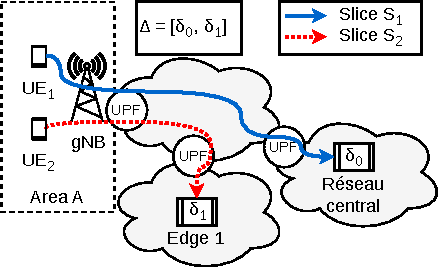
\includegraphics[width=\textwidth]{figs/01_00_evaluation-scenario-binding.drawio.pdf}
        \caption[]{Vue d’ensemble du réseau~5G déployé.}
        \label{fig:scenario-binding}
    \end{subfigure}
    \begin{subfigure}[t]{0.45\textwidth}
        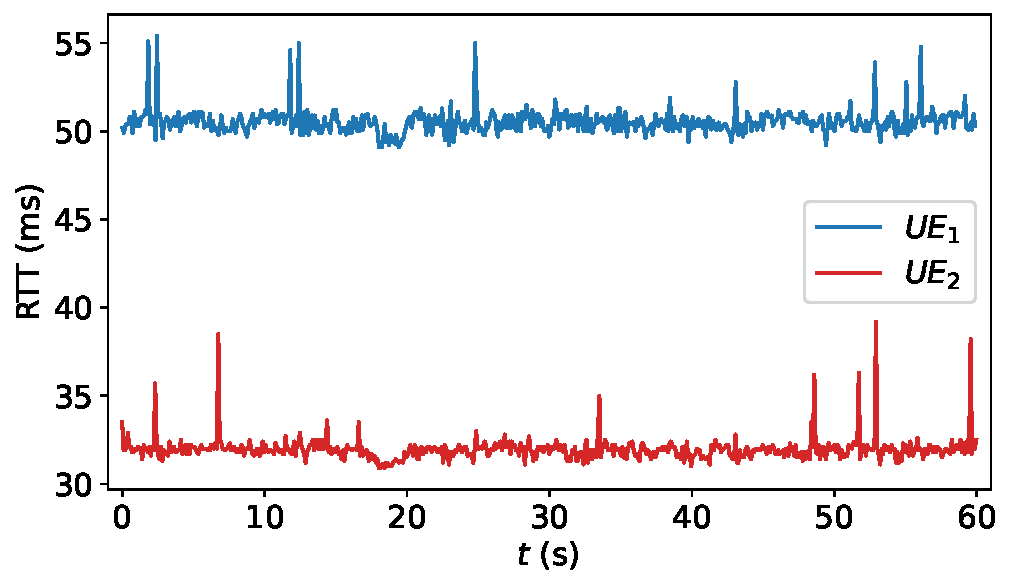
\includegraphics[width=\textwidth]{figs/01_10_evaluation-plot-binding.pdf}
        \caption[]{Mesure du \acren{RTT} avec le \gl{service/instances}{service}~$\Delta$ selon la \gl{slice}{\textit{slice}}.}
        \label{fig:evaluation-plot-binding}
    \end{subfigure}
    \caption[Mise en relation et accès avec des services \textit{edge} sur notre plateforme]{La politique~\textit{edge} met en relation l’UE\textsubscript{1} avec l’\gl{service/instances}{instance} $\delta_0$ dans le \gl{DN}{réseau de données} central (\gl{RTT}{RTT} > 50~ms), et l’UE\textsubscript{2} avec l’\gl{service/instances}{instance} $\delta_1$ dans l’\gl{edge}{\textit{edge}}~1 à proximité de l’\textit{area}~$A$ (\gl{RTT}{RTT} < 34~ms).}
    \label{fig:evaluation-binding}
\end{figure}

Nous établissons une \gl{PDU Session}{session~PDU} pour chacun des \gl{UE}{équipements}, et lançons simultanément deux mesures du \gl{RTT}{RTT} en envoyant des requêtes \textit{\gl{ICMP}{ICMP}~Echo} depuis les \gl{UE}{UEs} vers le \gl{service/instances}{service} $\Delta$ toutes les 100~ms pendant une minute.
La figure~\ref{fig:evaluation-plot-binding} montre que les politiques~\textit{edge} $P_1$ et $P_2$ (voir équation~\ref{eq:edge-policy-eval-binding}) sont bien respectées puisque le trafic est dirigé vers deux \gl{service/instances}{instances} différentes du même \gl{service/instances}{service}, l’une dans le réseau central, et l’autre dans l’\textit{edge}~1.

\pagebreak
\subsection{Changement d’instance~\textit{edge}}
Nous avons montré dans la section~\ref{sec:edge-instance-rebinding} que l’architecture~SR4MEC nous permet de changer d’\gl{service/instances}{instance}~\textit{edge} de manière transparente pour l’utilisateur.

Pour rappel, dans une architecture~5G classique avec des \gl{ULCL}{\textit{Uplink Classifiers} (ULCL)}, la sélection d’un \gl{edge}{\textit{edge}} spécifique pour un couple \gl{user}{utilisateur}/\gl{service/instances}{service} ne \gl{scalability}{passe pas à l’échelle} (voir section~\ref{sec:ULCL}).
Ainsi, si l’on souhaite effectuer un changement d’\gl{service/instances}{instance}, il faut considérer une approche moins granulaire en associant chaque \gl{PDU Session}{session~PDU} à un seul \gl{DN}{réseau de données} à la fois: soit un réseau central, soit un \gl{edge}{réseau~\textit{edge}}.
Pour effectuer un changement d’\gl{service/instances}{instance} en préservant la continuité de service, il est alors nécessaire que tous les \gl{service/instances}{services} utilisés soient instanciés dans l’\gl{edge}{edge} cible.

Avec l’architecture~SR4MEC, nous pouvons effectuer le changement d’une \gl{service/instances}{instance}~\textit{edge} particulière sans avoir à migrer vers l’\gl{edge}{\textit{edge}}~cible l’ensemble des autres \gl{service/instances}{services} utilisés.

Nous configurons notre plateforme avec deux \gl{edge}{\textit{edges}} et un \gl{DN}{réseau central} (voir figure~\ref{fig:evaluation-scenario-rebinding}), et y déployons deux \gl{service/instances}{services}, $\Delta$ et $\Omega$.
Nous déployons à la fois un \gl{CUPS}{plan de données}~5G classique et notre implémentation de l’architecture~SR4MEC, chaque architecture correspondant à un groupe de \gl{slice}{\textit{slices}}, et établissons une \gl{PDU Session}{session~PDU} pour chaque architecture.

\begin{figure}[h]
    \centering
    \begin{subfigure}[t]{0.45\textwidth}
        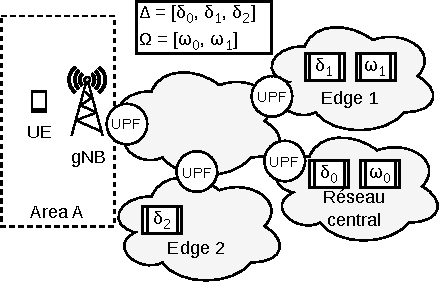
\includegraphics[width=\textwidth]{figs/02_00_evaluation-scenario-rebinding.drawio.pdf}
        \caption[]{Vue d’ensemble du réseau~5G déployé.}
        \label{fig:evaluation-scenario-rebinding}
    \end{subfigure}
    \begin{subfigure}[t]{0.45\textwidth}
        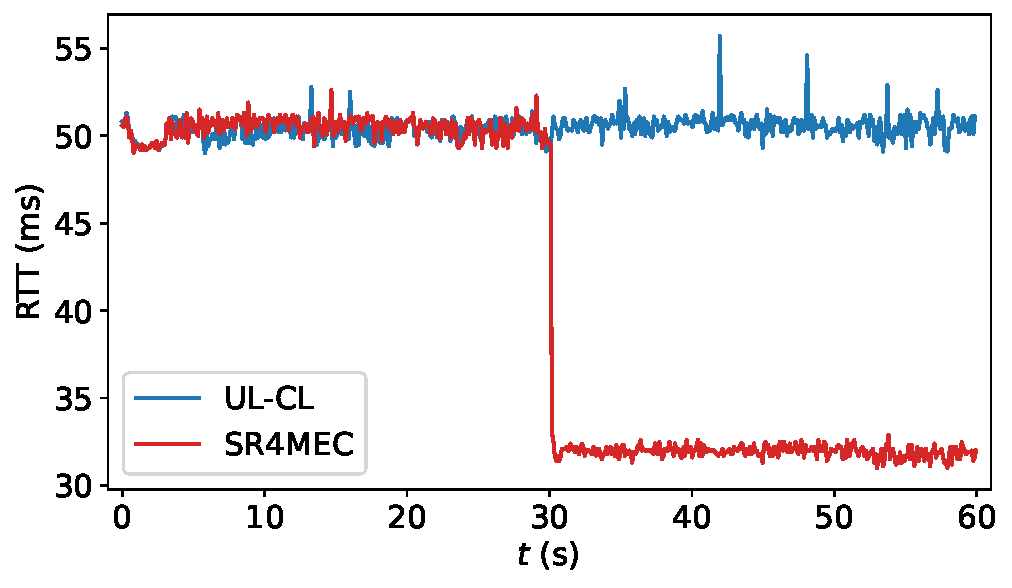
\includegraphics[width=\textwidth]{figs/02_10_evaluation-plot-rebinding.pdf}
        \caption[]{\gl{RTT}{RTT} avec un changement d’\gl{service/instances}{instance} à $t=30$.}
        \label{fig:evaluation-plot-rebinding}
    \end{subfigure}
    \label{fig:evaluation-rebinding}
    \caption[Changement d’instance \textit{edge} sur notre plateforme]{L’\gl{UE}{UE} accède initialement aux \gl{service/instances}{instances} $\delta_1$ et $\omega_1$ dans l’\gl{edge}{\textit{edge}}~1.}
\end{figure}

L’\gl{edge}{\textit{edge}}~2 est plus proche de l’\textit{area}~$A$ que l’\gl{edge}{\textit{edge}}~1, mais ne dispose initialement pas assez de ressources pour permettre de traiter les données de notre \gl{UE}{équipement utilisateur} (équation~\ref{eq:edge-policy-eval-rebinding-before}).
Des ressources sont par la suite libérées dans l’\gl{edge}{\textit{edge}~2} et réallouées à l’\gl{service/instances}{instance} $\delta_2$, si bien qu’à $t=30$ l’opérateur décide de mettre à jour sa politique \textit{edge} pour migrer notre équipement vers $\delta_2$ (équation~\ref{eq:edge-policy-eval-rebinding-after}).

\begin{subnumcases}{ Politique\ Edge =\label{eq:edge-policy-eval-rebinding}}
       P_1: S_1 \times A \times \Delta \rightarrow Edge\ 1 & (t\ <\ 30)\label{eq:edge-policy-eval-rebinding-before}\\
       P_1: S_1 \times A \times \Delta \rightarrow Edge\ 2 & (t\ \ge\ 30)\label{eq:edge-policy-eval-rebinding-after}
\end{subnumcases}

\pagebreak
Ce changement d’\gl{service/instances}{instance} peut être effectué lorsque l’\gl{UE}{UE} utilise un \gl{CUPS}{plan de données}~SR4MEC pour accéder au \gl{service/instances}{service}~$\Delta$, mais n’est pas autorisée avec l’architecture~5G classique.
Avec SR4MEC, le \gl{RTT}{RTT} moyen est initialement 50,448~ms puis lors du changement d’\gl{service/instances}{instance} il diminue pour atteindre 31,948~ms (voir figure \ref{fig:evaluation-plot-rebinding}), ce qui confirme que le trafic a bien été dirigé vers l’\gl{service/instances}{instance} $\delta_2$ dans l’\gl{edge}{\textit{edge}} le plus proche.
Au cours de notre expérience, comme le montre la capture~\ref{ping:rebinding}, aucun paquet n’est perdu pendant le changement d’\gl{service/instances}{instance} puisque l’ancien chemin descendant entre $\delta_1$ et l’\gl{UE}{UE} est préservé jusqu’à l’écoulement d’un délai suffisant.

\begin{lstlisting}[style=centercomments,label=ping:rebinding,caption=Ping vers le service~$\Delta$ avec l’architecture~SR4MEC pendant le changement d’\gl{service/instances}{instance}.,captionpos=b,frame=tb]
$ ping -D -w 60 10.4.0.1 -i 0.1 
PING 10.4.0.1 (10.4.0.1) 56(84) bytes of data.
[1776867821.303196] 64 bytes from 10.4.0.1: icmp_seq=1 ttl=63 time=50.6 ms
[1776867821.404007] 64 bytes from 10.4.0.1: icmp_seq=2 ttl=63 time=50.5 ms
[1776867821.505305] 64 bytes from 10.4.0.1: icmp_seq=3 ttl=63 time=50.9 ms

# ...

[1776867851.287572] 64 bytes from 10.4.0.1: icmp_seq=299 ttl=63 time=49.7 ms
[1776867851.387959] 64 bytes from 10.4.0.1: icmp_seq=300 ttl=63 time=49.3 ms
[1776867851.472194] 64 bytes from 10.4.0.1: icmp_seq=301 ttl=63 time=33.0 ms
[1776867851.572063] 64 bytes from 10.4.0.1: icmp_seq=302 ttl=63 time=32.6 ms

# ...

[1776867881.048403] 64 bytes from 10.4.0.1: icmp_seq=595 ttl=63 time=31.4 ms
[1776867881.149239] 64 bytes from 10.4.0.1: icmp_seq=596 ttl=63 time=31.6 ms
[1776867881.250563] 64 bytes from 10.4.0.1: icmp_seq=597 ttl=63 time=32.0 ms

--- 10.4.0.1 ping statistics ---
597 packets transmitted, 597 received, 0% packet loss, time 59966ms
rtt min/avg/max/mdev = 31.010/41.245/52.602/9.261 ms
\end{lstlisting}


\pagebreak
\subsection{Mobilité de l’utilisateur}
\label{sec:evaluation-mobility}

Dans le chapitre~\ref{ch:mobility}, nous avons proposé des procédures qui permettent à notre architecture~SR4MEC de prendre en compte la mobilité des utilisateurs.

Nous configurons notre plateforme pour utiliser NextMN Lite, et nous y ajoutons une deuxième \textit{area}.

Dans le réseau que nous déployons (figure~\ref{fig:evaluation-scenario-mobility}), le \gl{service/instances}{service}~$\Delta$ est instancié dans tous les \gl{DN}{réseaux de données}, mais le \gl{service/instances}{service}~$\Omega$ n’est pas instancié dans l’\gl{edge}{\textit{edge}}~2.


Puisque nous cherchons à observer l’impact des changements d’\gl{edge}{\textit{edge}} pendant la procédure de mobilité, nous devons configurer notre plateforme pour prendre en compte la latence entre nos différents équipements. 

\begin{figure}[h]
    \centering
    \begin{subfigure}[t]{0.45\textwidth}
        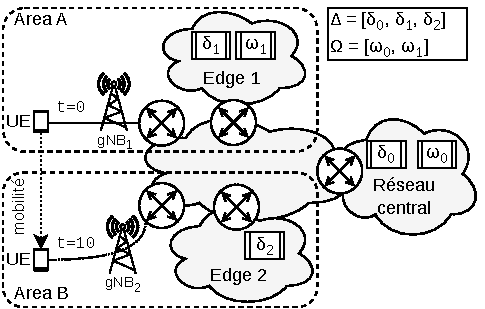
\includegraphics[width=\textwidth]{figs/03_00_evaluation-scenario-mobility.drawio.pdf}
        \caption[]{Scénario de mobilité au sein de notre réseau~5G.}
        \label{fig:evaluation-scenario-mobility}
    \end{subfigure}
    \begin{subfigure}[t]{0.45\textwidth}
        \centering
        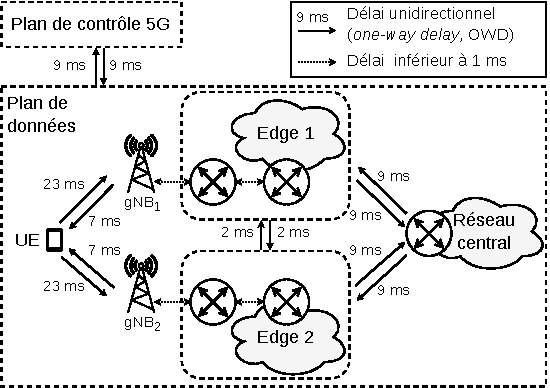
\includegraphics[width=\textwidth]{figs/03_01_evaluation-config-mobility.drawio.pdf}
        \caption[]{Configuration des latences entre les différentes zones de notre réseau~5G.}
        \label{fig:evaluation-config-mobility}
    \end{subfigure}
    \caption[Configuration de notre plateforme pour les scénarios de mobilité]{Notre réseau 5G est constitué de plusieurs zones géographiques distinctes: le \gl{CUPS}{plan de contrôle}, le réseau~central, l’\textit{area}~$A$ et l’\textit{area}~$B$.}
    \label{fig:evaluation-mobility}
\end{figure}

Dans notre scénario, l’\gl{edge}{\textit{edge}}~1 est co-localisé avec les équipements de l’\textit{area}~$A$, et l’\gl{edge}{\textit{edge}}~2 avec ceux de l’\textit{area}~$B$.
Le \acren{RTT} entre les deux \textit{areas} est égal à 4~ms.

L’utilisateur accède aux \gl{gNB}{gNBs} en utilisant une liaison radio~5G.
Concernant les latences radio, nous nous fondons sur des mesures issues d’un \gl{SA}{réseau~5G~\textit{Standalone}} privé déployé sur le campus de l’Université de Toulouse~\cite{10.1109/WoWMoM69805.2026.00018}, ainsi que sur \cite{10.70675/d8048253zf45fz4136z9c3fz3cf364403791} qui montre également une asymétrie entre les liens radio montants et descendants.
Dans ces travaux, le \acren{RTT} moyen est de 30~ms entre l’\gl{UE}{UE} et un \gl{service/instances}{service~edge}, la contribution en latence du segment \gl{gNB}{gNB}/\gl{edge}{\textit{edge}} étant considérée comme négligeable devant celle du lien radio.

Nous configurons les interfaces réseaux entre ces différentes zones en utilisant l’outil \textit{Traffic Control}~(\texttt{tc}) du projet Linux afin de reproduire des latences réalistes que nous détaillons sur la figure~\ref{fig:evaluation-config-mobility}. 
Dans nos mesures, les \gl{RTT}{RTTs} relevés sont supérieurs à la somme des délais unidirectionnels indiqués sur cette figure car il faut y ajouter le temps de traitement des \gl{PDU}{PDUs} par les différents conteneurs.


\pagebreak
\subsubsection{Mobilité avec une architecture 5G classique}
Dans cette section, nous illustrons d’abord le déroulement de la mobilité \textit{inter-areas} avec une architecture~5G classique, qui ne permet pas le changement d’\gl{edge}{\textit{edge}}.

Puis, dans les sections~\ref{sec:testbed-mobility-changement-a-posteriori} et \ref{sec:testbed-mobility-changement-immediat}, nous utiliserons l’architecture~SR4MEC dans des scénarios où cette mobilité cause le changement d’\gl{service/instances}{instance}, et montrerons que le choix de la procédure de mobilité a un impact sur l’évolution de la latence.

\begin{figure}[h]
    \centering
    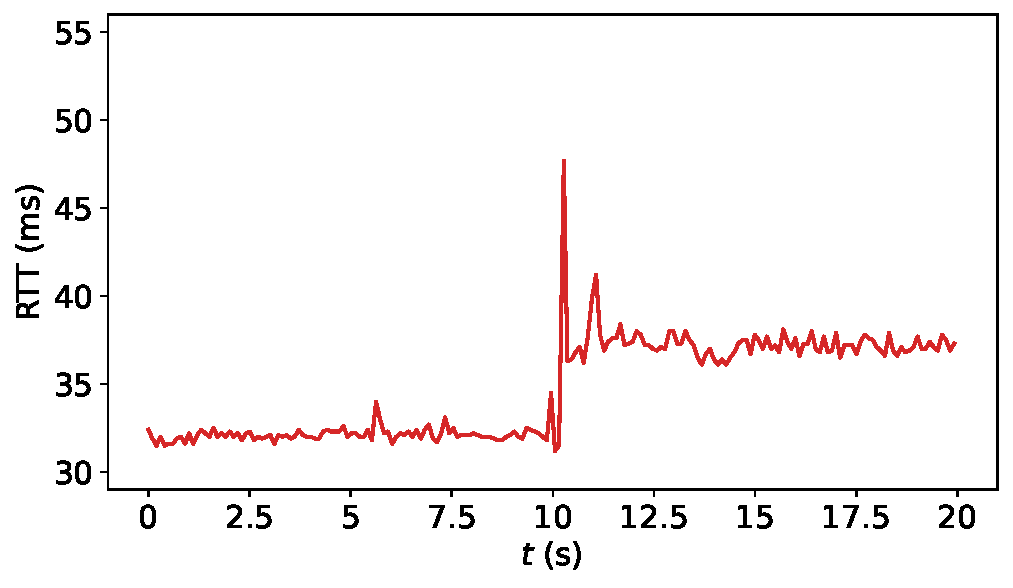
\includegraphics[width=0.75\textwidth]{figs/03_10_evaluation-plot-mobility-ulcl.pdf}
    \caption[Mobilité avec une architecture 5G classique]{\acren{RTT} avec une architecture~5G classique. À $t=0$, l’\gl{user}{utilisateur} se situe dans l’\textit{area}~A, puis il se déplace vers l’\textit{area}~B à $t=10$.}
    \label{fig:evaluation-plot-mobility-ulcl}
\end{figure}

Dans la figure~\ref{fig:evaluation-plot-mobility-ulcl}, à partir de $t=0$ et durant toute la session, l’utilisateur utilise les \gl{service/instances}{instances} $\delta_1$~et~$\omega_1$.
On ne peut pas faire de changement d’\gl{service/instances}{instance} puisqu’il n’est pas possible de changer d’\gl{service/instances}{instance} pour les \gl{service/instances}{services} utilisés vers l’\gl{edge}{\textit{edge}}~2 (cet \gl{edge}{\textit{edge}} ne permet pas le déploiement d’une \gl{service/instances}{instance} de $\Omega$).

À l’instant $t=10$, l’\gl{user}{utilisateur} se déplace vers l’\textit{area}~B, la procédure de \gl{handover}{\textit{handover}} vers la \gl{gNB}{gNB\textsubscript{2}} se déclenche, et nous observons une augmentation du \acren{RTT}, initialement environ à 33~ms, pour atteindre environ~37~ms.

Lorsque la \gl{gNB}{gNB}~source reçoit le message \texttt{Handover Command} du \gl{CUPS}{plan de contrôle}~5G, les réponses~\gl{ICMP}{ICMP} sont transmises vers la \gl{gNB}{gNB}~cible en utilisant le chemin de \textit{forwarding} (ici, entre \gl{gNB}{gNB\textsubscript{1}} et \gl{gNB}{gNB\textsubscript{2}}).
Ces messages sont ensuite placés en file d’attente jusqu’à la synchronisation de l’\gl{UE}{équipement utilisateur}, ce qui produit un pic dans la mesure du \gl{RTT}{RTT} (47.7~ms).
Une fois le \gl{handover}{\textit{handover}} terminé, le \gl{RTT}{RTT} se stabilise à environ 37~ms car l'utilisateur continue d’accéder aux \gl{service/instances}{instances} de l'\gl{edge}{\textit{edge}}~1 mais maintenant à partir de l'\textit{area}~B.

\pagebreak
\subsubsection{Mobilité avec changement d’instance \textit{a posteriori}}
\label{sec:testbed-mobility-changement-a-posteriori}
Contrairement à l’architecture~5G classique, notre architecture~SR4MEC permet le changement d’\gl{service/instances}{instance~\textit{edge}} de manière indépendante pour chaque \gl{service/instances}{service}.

Lorsque la mobilité de l’utilisateur est effectuée sans anticiper suffisamment tôt le changement d’\gl{service/instances}{instance}, il reste possible d’effectuer ce changement \textit{a posteriori}, comme l’illustre la figure~\ref{fig:evaluation-plot-mobility-changement-a-posteriori} où la décision de changement d’\gl{service/instances}{instance} vers $\delta_2$ est prise 3~secondes après la fin du \gl{handover}{\textit{handover}}.

Sur la figure~\ref{fig:evaluation-plot-mobility-changement-a-posteriori-central}, l’\gl{user}{utilisateur} accède initialement à l’\gl{service/instances}{instance} centrale $\delta_0$.
Le \acren{RTT} moyen initial est de 50,8~ms.
Puisque le changement d’\gl{service/instances}{instance} n’est pas immédiat et que la latence entre le réseau central et les différentes \textit{areas} est identique, nous n’observons pas de différence significative après le \gl{handover}{\textit{handover}}~($t = 10$), hormis un pic (51,9~ms) dû au \textit{forwarding} entre l’\textit{area}~A et l’\textit{area}~B.
Une fois le changement d’\gl{service/instances}{instance} effectué, le \acren{RTT} moyen est réduit à 32~ms, montrant que le changement d’instance a bien pu se réaliser.

\begin{figure}[h]
    \centering
    \begin{subfigure}{0.45\textwidth}
        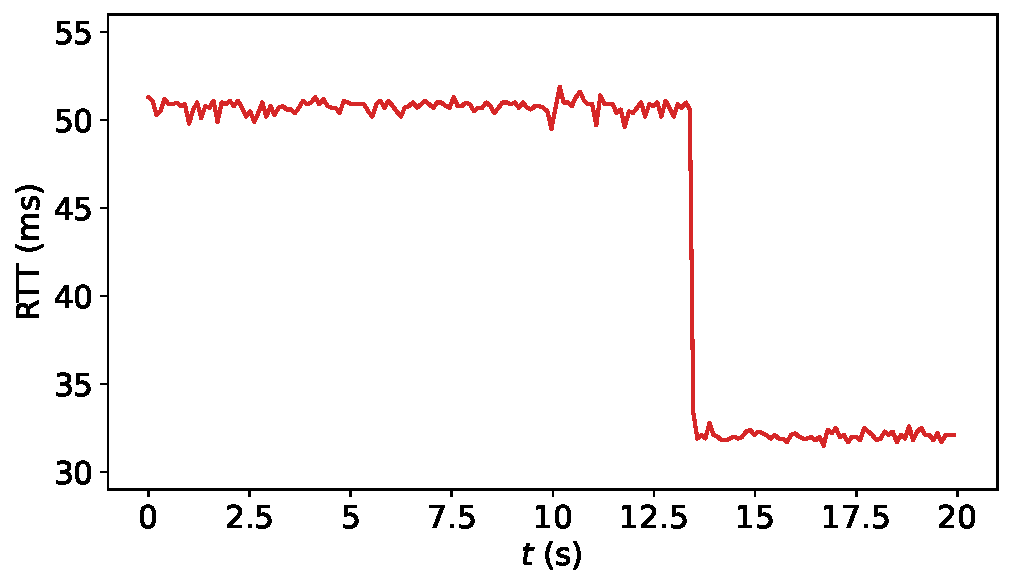
\includegraphics[width=\textwidth]{figs/03_20_evaluation-plot-mobility-changement-a-posteriori-central.pdf}
        \caption[]{Relation initiale: $\delta_0$}
        \label{fig:evaluation-plot-mobility-changement-a-posteriori-central}
    \end{subfigure}
    \begin{subfigure}{0.45\textwidth}
        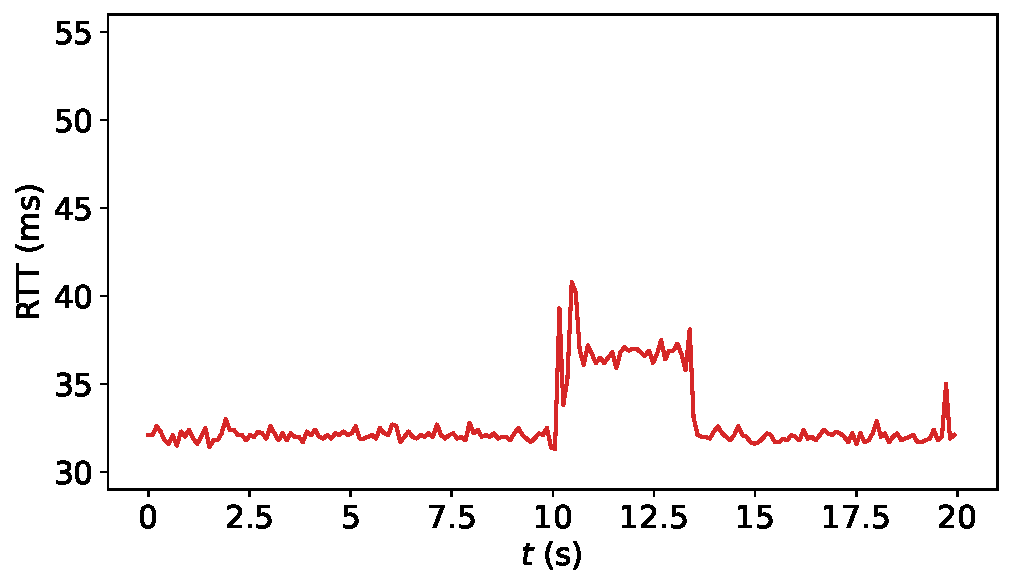
\includegraphics[width=\textwidth]{figs/03_21_evaluation-plot-mobility-changement-a-posteriori-edge.pdf}
        \caption[]{Relation initiale: $\delta_1$}
        \label{fig:evaluation-plot-mobility-changement-a-posteriori-edge}
    \end{subfigure}
    \caption[Mobilité avec changement d’instance \textit{a posteriori} (SR4MEC)]{À $t=10$ le \gl{handover}{\textit{handover}} est déclenché en préservant la relation entre l’\gl{UE}{UE} et l’\gl{service/instances}{instance} initiale. Un changement d’\gl{service/instances}{instance} est effectué \textit{a posteriori} (ici, 3~s après le \gl{handover}{\textit{handover}}).}
    \label{fig:evaluation-plot-mobility-changement-a-posteriori}
\end{figure}

Sur la figure \ref{fig:evaluation-plot-mobility-changement-a-posteriori-edge}, nous présentons un scénario alternatif où l’\gl{user}{abonné} accède initialement à l’\gl{service/instances}{instance}~$\delta_1$, situé dans un \gl{edge}{\textit{edge}} a proximité.
Le \acren{RTT} initial est donc de 32~ms.
Puisque les \gl{edge}{\textit{edges}}~1 et 2 sont distants de 4~ms, la mobilité de l’utilisateur augmente la latence entre l’\gl{UE}{UE} et $\delta_1$.
Le changement d’\gl{service/instances}{instance} est effectif à partir de $t=13,5$ et il permet de restaurer la latence initiale.

Ces deux exemples illustrent l’intérêt d’intégrer la détection des événements de mobilité dans le processus de mise en relation: lorsqu’une \gl{service/instances}{instance} centrale est initialement utilisée, la mobilité peut rapprocher l’utilisateur d’une \gl{service/instances}{instance \textit{edge}}, rendant son usage suffisamment attractif pour justifier un changement \gl{service/instances}{instance}; et à l’inverse lorsqu’une \gl{service/instances}{instance} d’un \gl{edge}{\textit{edge}} local est utilisée, on souhaitera maintenir la \gl{QoS}{qualité de service} initiale en utilisant l’\gl{edge}{\textit{edge}} devenu le plus proche.

\pagebreak
\enlargethispage*{1\baselineskip} % pour éviter 1 ligne orpheline à la fin de la page
\subsubsection{Mobilité avec changement d’instance immédiat}
\label{sec:testbed-mobility-changement-immediat}

Lorsque la mobilité de l’utilisateur est prévisible et qu’il a été déterminé au préalable qu’un changement d’\gl{service/instances}{instance} est pertinent, l’architecture~SR4MEC nous permet d’effectuer ce changement d’\gl{service/instances}{instance} au cours du \gl{handover}{\textit{handover}}.
En comparaison avec un changement d’instance \textit{a posteriori}, cette procédure de mobilité que nous avons proposé dans la section~\ref{sec:mobility-with-immediate-intance-update} présente un avantage double: les messages de contrôles sont moins nombreux, et l’accès à l’\gl{service/instances}{instance}~cible coïncide avec le changement de \gl{gNB}{station de base}, comme le montre la figure~\ref{fig:evaluation-plot-mobility-changement-immediat}.
Contrairement au scénario avec changement \textit{a posteriori}, les chemins pour accéder à l’\gl{service/instances}{instance}~$\delta_2$ sont créés pendant la phase de préparation du \gl{handover}{\textit{handover}}, ce qui permet son utilisation dès le début de la phase d’exécution, et avant même la réception du message \texttt{Handover Notify} par le \gl{CUPS}{plan de contrôle}~5G.

Sur la figure~\ref{fig:evaluation-plot-mobility-changement-immediat-central}, l’\gl{user}{abonné} utilise initialement l’\gl{service/instances}{instance}~$\delta_0$ dans le réseau central.
À $t=10$, l’\gl{user}{abonné} se déplace sur la \gl{gNB}{gNB\textsubscript{2}} dans l’\textit{area}~B; le \gl{RTT}{RTT} vers le service $\Delta$ chute à environ 32~ms, montrant que le changement d’\gl{service/instances}{instance} s’est fait pendant la procédure de \gl{handover}{\textit{handover}}.

\begin{figure}[h]
    \centering
    \begin{subfigure}{0.45\textwidth}
        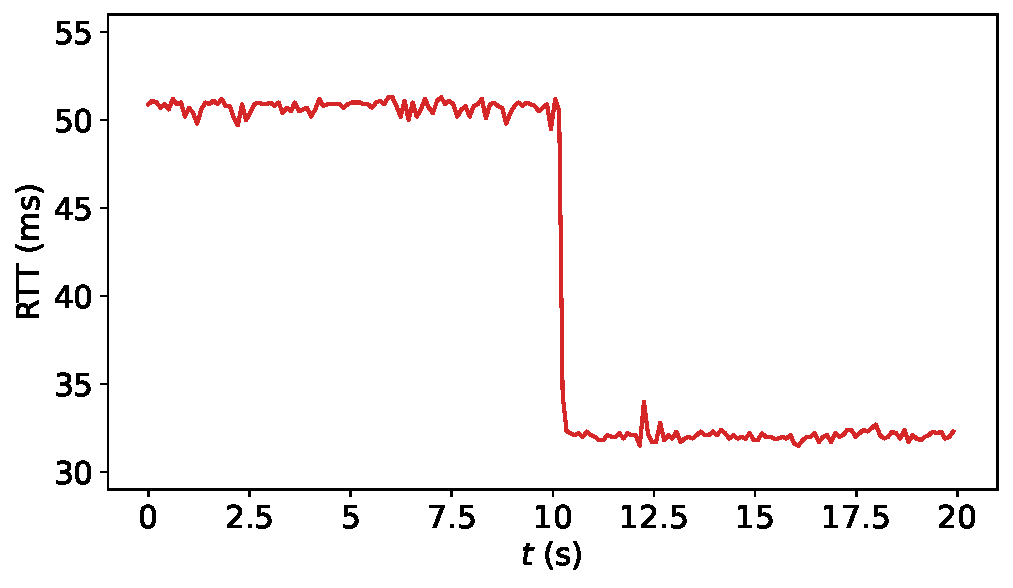
\includegraphics[width=\textwidth]{figs/03_30_evaluation-plot-mobility-changement-immediat-central.pdf}
        \caption[]{Relation initiale: $\delta_0$}
        \label{fig:evaluation-plot-mobility-changement-immediat-central}
    \end{subfigure}
    \begin{subfigure}{0.45\textwidth}
        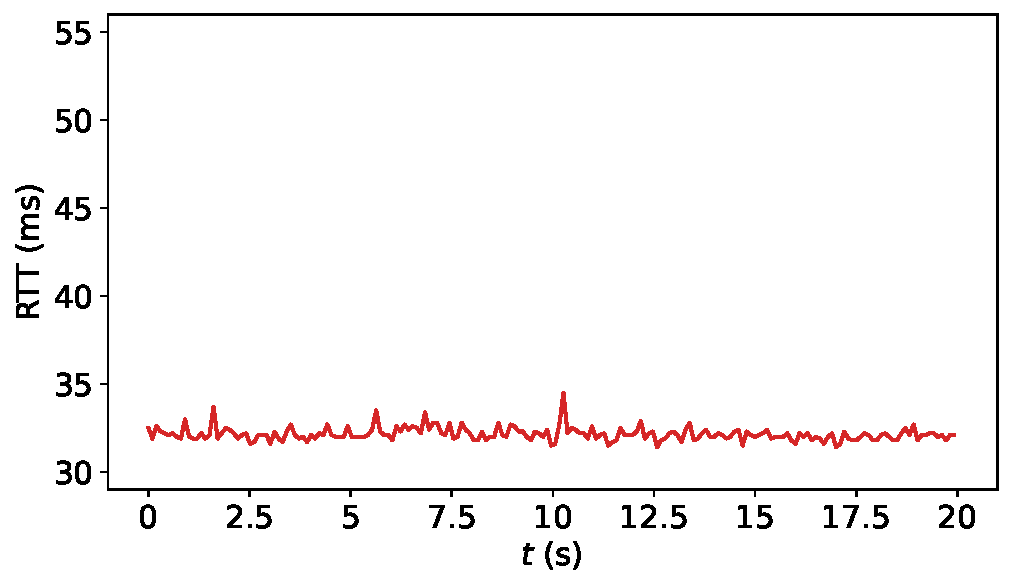
\includegraphics[width=\textwidth]{figs/03_31_evaluation-plot-mobility-changement-immediat-edge.pdf}
        \caption[]{Relation initiale: $\delta_1$}
        \label{fig:evaluation-plot-mobility-changement-immediat-edge}
    \end{subfigure}
    \caption[Mobilité avec changement d’instance immédiat (SR4MEC)]{À $t=10$, le \gl{handover}{\textit{handover}} est déclenché, et résulte en un changement immédiat d’\gl{service/instances}{instance}.}
    \label{fig:evaluation-plot-mobility-changement-immediat}
\end{figure}

Sur la figure~\ref{fig:evaluation-plot-mobility-changement-immediat-edge}, l’\gl{user}{utilisateur} accède initialement à l’\gl{service/instances}{instance} $\delta_1$, et lors de la mobilité nous faisons un changement immédiat d’\gl{service/instances}{instance} afin de maintenir un \gl{RTT}{RTT} faible.
Le \acren{RTT} moyen est 32,148~ms avec un écart type de~0,386~ms.
Nous mesurons un \acren{RTT} maximum lors de l’utilisation du chemin de \textit{forwarding}~(34,545~ms).

Avec ce dernier scénario, à tout moment l’instance optimale est utilisée, si bien que le \gl{handover}{\textit{handover}} et le changement d’\gl{service/instances}{instance} deviennent transparents pour l’\gl{user}{utilisateur}.

\section{Synthèse}

Dans ce chapitre, nous avons présenté notre plateforme d’expérimentation et ses différents modules qui permettent le déploiement d’un réseau~5G réel et son intégration à l’\textit{edge computing}.
Nous avons apporté des preuves fonctionnelles en testant et comparant une implémentation de notre architecture~SR4MEC avec une architecture~5G classique, et montré son gain en matière d’accès à des \gl{service/instances}{instances de service} proches de l’\gl{user}{utilisateur} à la fois lors de l’établissement de la \gl{PDU Session}{session~PDU} mais aussi lors de changements dynamiques suite à une décision de l’opérateur ou à une mobilité de l’\gl{user}{utilisateur}.

\end{document}